
\section{Characterization of the I-V-Curves}\label{sec:charac}

In order to characterize the assembled sets of \BHSC's, we used the Keithley~2602A~Sourcemeter and ABET~Technologies’ solar simulator SUN~2000. The simulator reproduces the AM 1.5 global reference spectrum and was also equipped with 5 different filters for varying the light intensity. Using the source meter we applied sequences of voltages to the cells and measured the currents resulting from their irradiation. This was done at different levels of intensity of light as well as darkness for which we covered each set with a plastic box.
\subsection{Irradiance calibration}
To ensure that the SUN~2000 was calibrated to yield an irradiance of $1\;\text{mW}\!\cdot\text{mm}^{-2}$, we used the Laser~Point PD-500-D9-VIS. With a digital caliper we measured the aperture of the photo diode to have a diameter of $d_p = 9.9(5)\;\text{mm}$. Here we had to assume such a high uncertainty because the construction of the aperture made it very difficult to make out the diameter. This yields an irradiated area of
\begin{equation*}
A_p =  77(8)\;\text{mm}^2.
\end{equation*}
The total power $P_{p0}$ measured by the photo diode at maximum\footnote{This is the intensity corresponding to no filter. We will refer to it with the index 0.} intensity yielded $P_{p0} = 82(1)\;\text{mW}$. So that we arrive at an irradiance of
\begin{equation*}
S_{p0} = 1.07(11)\;\frac{\text{mW}}{\text{mm}^2}.
\end{equation*}
As we will show in section~\ref{sec:improvements} there is external information (see \cite{photodiode}) on the aperture of the photo diode we could not make out at the time of the lab.
\begin{figure}[h]
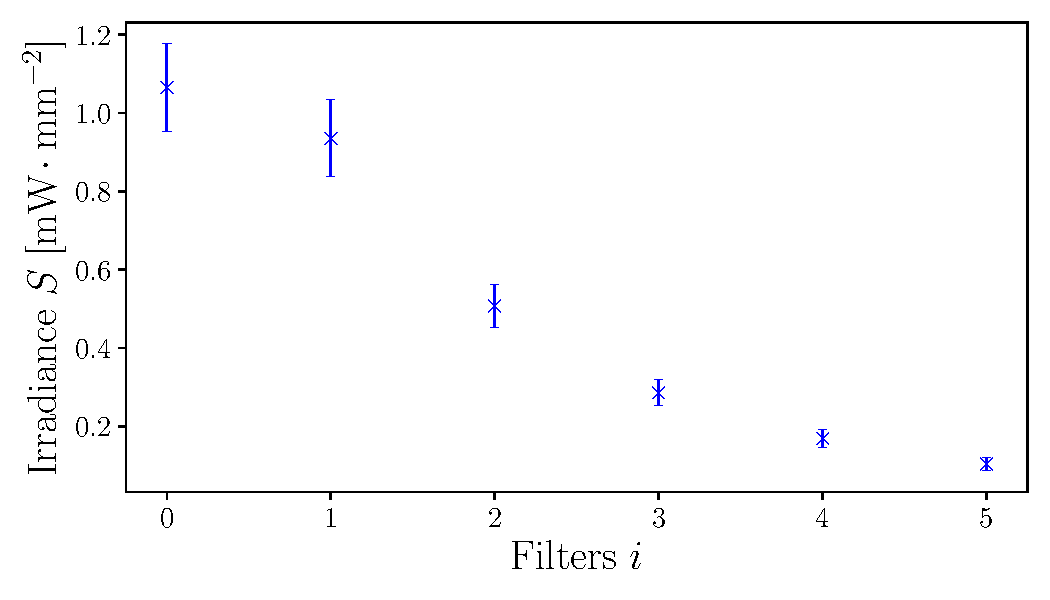
\includegraphics[scale=0.5]{../2_Pictures/Photodiode_irradiance.pdf}
\caption{Measured irradiances $S_{pi}$ for each filter $i$ with Laser~Point PD-500-D9-VIS.}
\label{fig:photodiode_irradiances}
\end{figure}

We also conducted this measurement with all filters available to us, in order to see how they modulate the intensity of the light. As we can deduct from figure~\ref{fig:photodiode_irradiances}, each filter does not modulate the lights intensity in a linear fashion.\mypar
We were aware of the uncertainty in the measurements provided by the photo diode. Hence we performed additional measurements of I-V-curves using a Rera~RQN3686 silicon reference cell. This cell was calibrated on the AM 1.5 spectrum, so in order to check if our solar simulator was calibrated correctly we compared our measurements with the reference values (see \cite{reracat}) illustrated in table~\ref{tab:reracomp}. Because of no uncertainties given in the reference values, we are going to assume an error equal to a single unit in the last figure quoted (see \cite{measurements} section 2.8.1). For the determination of the uncertainty of our measured values we used the same methods as described in the section~\ref{subsec:calckeyparams} below.
\begin{table}[h]\centering
\caption{Comparison of our measurements with the reference values of the Rera~RQN3686 silicon reference cell for calibration purposes.}
\label{tab:reracomp}
\begin{tabular}{@{}lcc@{}}\toprule
Quantity & Reference value & Measured value\\ \midrule
$\jsc$ [mA$\cdot$cm$^{-2}$] & 32.7(1) & 32.783(16) \\
$\Uoc$ [mV]& 596(1) & 596.3(4) \\ \bottomrule
\end{tabular}
\end{table}

It is evident from table~\ref{tab:reracomp} that our measured results are deficient in accuracy but yield a better precision than those referenced. But nonetheless both of our measured values lie within the range of one $\sigma$ of the values specified by the manufacturer from which we conclude that the SUN~2000 was calibrated correctly.


\subsection{Calculation of key parameters}\label{subsec:calckeyparams}
In order to calculate the open circuit voltage $\Uoc$ and the short circuit current density $\jsc$ for a set of measurements, we performed two linear interpolations.

 between the two closest points to the relevant axis\footnote{Being the $j$-axis for $\Uoc$ and the $U$-axis for $\jsc$.}, on each side of it. So if our chosen points for the calculation of $\Uoc$ are $\{(j_1,U_1),(j_2,U_2)\}$ and for $\jsc$ are $\{(j_1^\prime,U_1^\prime),(j_2^\prime,U_2^\prime)\}$, then the formulas for $\Uoc$ and $\jsc$ are as follows.
\begin{align}
\Uoc = \frac{U_2 j_1 - U_1 j_2}{j_1-j_2}\quad \jsc = \frac{U_1^\prime j_2^\prime - U_2^\prime j_1^\prime}{U_1^\prime-U_2^\prime}
\end{align}

To get the maximum power density we simply multiplied the current densities and voltages and took the largest value.
\begin{align}
\Pmax = \max_{i} (j_i\cdot U_i)
\end{align}

The fill factor $FF$ is defined as the ratio of maximum power to the product of open circuit voltage and short circuit current.
\begin{align}
FF = \frac{\Pmax}{\Uoc \cdot \jsc}
\end{align}

Finally the maximum power conversion efficiency $\eta$ is defined as the ratio of maximum power density to the irradiance of the incident light.
\begin{align}
\eta = \frac{\Pmax}{S_p}
\end{align}

In the case of sets $\mathbb{S}_3$ and $\mathbb{S}_\star$ we had multiple working cells. For these we decided to do all calculations with the mean of the current density over the working cells $n$ and include the standard deviation in the uncertainties of our results. The systematic errors of the current $u_{I,\text{sys}}$ and voltage $u_{U,\text{sys}}$ measurements were taken from \cite{keithley}. The uncertainty of the mean of the current density of measurement pair $p$ then is given as:
\begin{align}
u_{\meann{j_p}} = \sqrt{\frac{\sigma_{j,p}^2}{N} + \meann{u_{j_p,\text{sys}}}^2}
\end{align}

With sample size $N$ being the amount of working cells of the set and the systematic error:
\begin{align}
u_{j_{pn},\text{sys}} = \sqrt{ \left( \frac{ u_{I_{pn},\text{sys}}}{A_n}\right)^2+\left( j_{pn}\frac{u_{A_n}}{A_n} \right)^2}
\end{align}

The uncertainties of the other parameters can then be obtained through Gaußian error propagation.

\subsection{First set of \BHSC s}\label{subsec:S1data}

For the first set of \BHSC s $\mathbb{S}_1$, for which only one cell was not shorted, we obtained the following parameters in descending order of light intensity.
%\begin{table}[H]\centering
% \caption{Key parameters for set $\mathbb{S}_1$ of \BHSC s}
% \label{tab:keyparams1}
% \begin{tabular}{@{}ccccc@{}}\toprule
% $i$ & $\Pmax$ [\textmu W cm$^{-2}$] & $\jsc$ [\textmu A $\mathrm{cm}^{-2}$] & $\Uoc$ [mV] & $FF$ [\%]\\\midrule
% 0 &  $ 22.1(12) $ & $ -149(5) $ & 424.6(4) & 34.9(21) \\
% 1 &  $ 15.9(9) $ & $ -124(4) $ & 387.6(3) & 33.0(22) \\
% 2 &  $ 9.6(5) $ & $ -70.0(24) $ & 343.7(4) & 31.7(23) \\
% 3 &  $ 2.55(21) $ & $ -37.0(13) $ & 235.2(4) & 29.3(26) \\
% 4 &  $ 0.75(9) $ & $ -19.7(7) $ & 131.3(3) & 29(4)\\
% 5 &  $ 0.18(5) $ & $ -10.5(4) $ & 70.93(22) & 24(6) \\
% \end{tabular}
%\end{table}
%\begin{table}[h]
% \centering
% \begin{tabular}{@{}ccc@{}}
% i & irradiance $S_{pi} []$
% \end{tabular}
%\end{table}

\begin{table}[h]
\begin{tabular}{@{}cccc@{}}
\toprule
\multicolumn{1}{c}{$\Pmax$ [\textmu W cm$^{-2}$]} & $\jsc$ [\textmu A $\mathrm{cm}^{-2}$] & \multicolumn{1}{c}{$\Uoc$ [mV]} & $FF$ [\%] \\ \midrule
\multicolumn{1}{c}{$ 22.1(12) $}                  & $ -149(5) $                           & \multicolumn{1}{c}{424.6(4)}    & 34.9(21)  \\
\multicolumn{1}{c}{$ 15.9(9) $}                   & $ -124(4) $                           & \multicolumn{1}{c}{387.6(3)}    & 33.0(22)  \\
\multicolumn{1}{c}{$ 9.6(5) $}                    & $ -70.0(24) $                         & \multicolumn{1}{c}{343.7(4)}    & 31.7(23)  \\
\multicolumn{1}{c}{$ 2.55(21) $}                  & $ -37.0(13) $                         & \multicolumn{1}{c}{235.2(4)}    & 29.3(26)  \\
\multicolumn{1}{c}{$ 0.75(9) $}                   & $ -19.7(7) $                          & \multicolumn{1}{c}{131.3(3)}    & 29(4)     \\
\multicolumn{1}{c}{$ 0.18(5) $}                   & $ -10.5(4) $                          & \multicolumn{1}{c}{70.93(22)}   & 24(6)     \\ \midrule
\multicolumn{2}{c}{$S_{pi}$ [mW mm$^{-2}$]}                                               & \multicolumn{2}{c}{$\eta$ [\%]}             \\\midrule
\multicolumn{2}{c}{1.06(11)}                                                              & \multicolumn{2}{c}{0.0207(24)}              \\
\multicolumn{2}{c}{0.94(10)}                                                              & \multicolumn{2}{c}{0.0170(20)}              \\
\multicolumn{2}{c}{0.51(5)}                                                               & \multicolumn{2}{c}{0.0151(19)}              \\
\multicolumn{2}{c}{0.29(3)}                                                               & \multicolumn{2}{c}{0.0089(13)}              \\
\multicolumn{2}{c}{0.169(22)}                                                             & \multicolumn{2}{c}{0.0045(8)}               \\
\multicolumn{2}{c}{0.104(17)}                                                             & \multicolumn{2}{c}{0.0017(5)}               \\ \bottomrule
\end{tabular}
\end{table}


In the following figure the current density measurements for four light intensities are shown. The blue rectangle indicates the short circuit current and the open circuit voltage and the orange rectangle the maximum power per area for the measurement at full intensity of incident light.

\begin{figure}[h]\centering
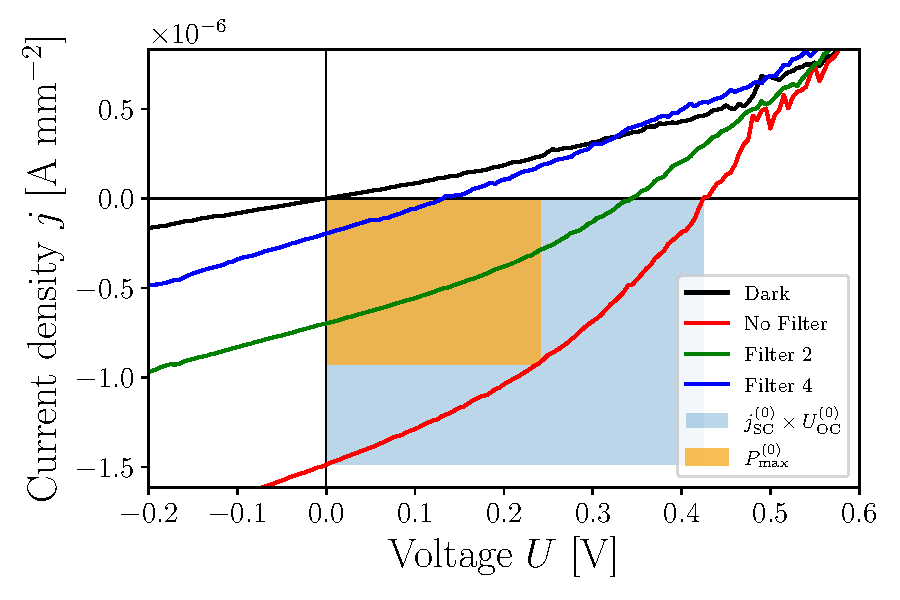
\includegraphics[width=\columnwidth]{../../../IV-Curve-Analysis/OSC1Graph.pdf}
\caption{Current density measurements for the set $\mathbb{S}_1$}
\label{fig:OSC1Graph}
\end{figure}

\subsection{Third set of \BHSC s}

The calculated key parameters for the third set of cells $S_3$, which have the same architecture as set $S_1$ are presented in the same way as in $\ref{subsec:S1data}$.

\begin{table}[h]
\begin{tabular}{@{}cccc@{}}
\toprule
$\Pmax$ [$\mu$W cm$^{-2}$] & $\jsc$ [$\mu$A $\mathrm{cm}^{-2}$] & $\Uoc$ [mV]     & $FF$ [\%]     \\ \midrule
16.2(14)                   & -111(6)                            & 515(5)          & 28.2(29)      \\
13.5(13)                   & -95(5)                             & 505(5)          & 28(3)         \\
7.4(6)                     & -52.7(27)                          & 478.9(24)       & 29.3(29)      \\
4.0(3)                     & -28.1(14)                          & 455.1(29)       & 31(3)         \\
2.11(17)                   & -15.0(8)                           & 431.2(20)       & 33(3)         \\
1.11(9)                    & -8.0(4)                            & 406.44(27)      & 34(3)         \\ \midrule
\multicolumn{2}{c}{$S_p$ [mW mm$^{-2}$]}                        & \multicolumn{2}{c}{$\eta$ [\%]} \\ \midrule
\multicolumn{2}{c}{1.06(11)}                                    & \multicolumn{2}{c}{0.0152(21)}  \\
\multicolumn{2}{c}{0.94(10)}                                    & \multicolumn{2}{c}{0.0144(20)}  \\
\multicolumn{2}{c}{0.51(5)}                                     & \multicolumn{2}{c}{0.0146(20)}  \\
\multicolumn{2}{c}{0.29(3)}                                     & \multicolumn{2}{c}{0.0139(19)}  \\
\multicolumn{2}{c}{0.169(22)}                                   & \multicolumn{2}{c}{0.0125(19)}  \\
\multicolumn{2}{c}{0.104(17)}                                   & \multicolumn{2}{c}{0.0107(19)}  \\ \bottomrule
\end{tabular}
\end{table}


\begin{figure}[h]\centering
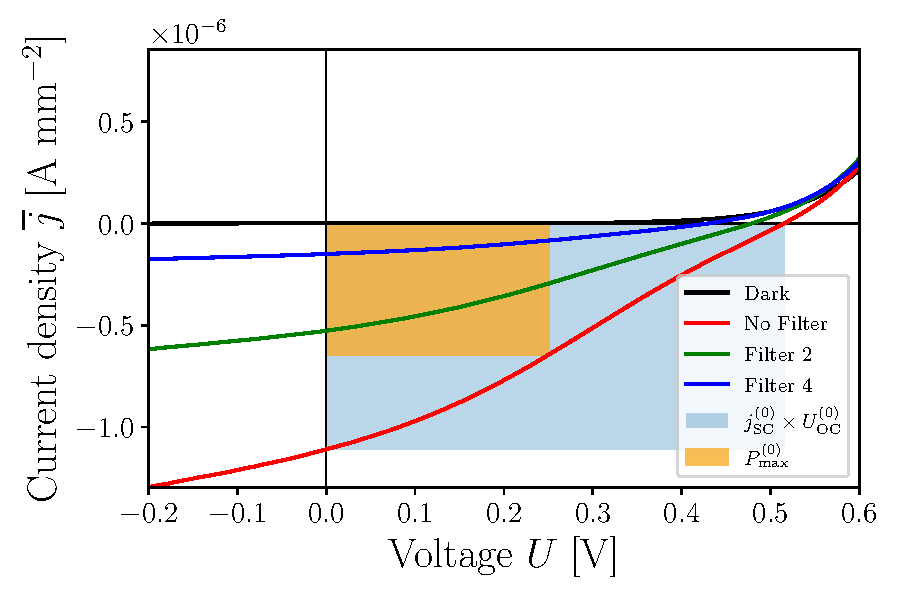
\includegraphics[width=\columnwidth]{../../../IV-Curve-Analysis/OSC2Graph.pdf}
\caption{Current density measurements for the set $\mathbb{S}_3$}
\label{fig:OSC3Graph}
\end{figure}

\subsection{Preassembled set of \BHSC s}

For this set of cells we did not measure the size of the Galinstan droplets, so in order to do the same calculations, we used the average of the measured areas and the average uncertainty as well $A_\star = \langle A_{kn} \rangle_{kn}$, $u_{A_\star} = \langle u_{A_{kn}}  \rangle_{kn}$. Because of this we can't really trust the exact values of the data, but the shape should remain the same.
\begin{table}[]
\begin{tabular}{@{}cccc@{}}
\toprule
$\Pmax$ [$\mu$W cm$^{-2}$] & $\jsc$ [$\mu$A $\mathrm{cm}^{-2}$] & $\Uoc$ [mV]          & $FF$ [\%]         \\ \midrule
10.4(12)                   & -49(3)                             & 747(6)               & 28(3)             \\
8.2(8)                     & -41.4(22)                          & 716(8)               & 27.7(29)          \\
4.7(4)                     & -23.7(12)                          & 704(7)               & 28.4(29)          \\
2.60(23)                   & -12.8(7)                           & 692(8)               & 29(3)             \\
1.43(13)                   & -7.0(3)                            & 694(7)               & 30(3)             \\
0.75(7)                    & -3.73(21)                          & 651(10)              & 31(4)             \\ \midrule
\multicolumn{2}{c}{$S_p$ [mW mm$^{-2}$]}                        & \multicolumn{2}{c}{$\eta$ [\%]} \\ \midrule
\multicolumn{2}{c}{1.06(11)}                                    & \multicolumn{2}{c}{0.0097(15)}           \\
\multicolumn{2}{c}{0.94(10)}                                    & \multicolumn{2}{c}{0.0088(12)}           \\
\multicolumn{2}{c}{0.51(5)}                                     & \multicolumn{2}{c}{0.0094(13)}           \\
\multicolumn{2}{c}{0.29(3)}                                     & \multicolumn{2}{c}{0.0091(13)}           \\
\multicolumn{2}{c}{0.169(22)}                                   & \multicolumn{2}{c}{0.0084(13)}           \\
\multicolumn{2}{c}{0.104(17)}                                   & \multicolumn{2}{c}{0.0073(13)}           \\ \bottomrule
\end{tabular}
\end{table}


\begin{figure}[H]\centering
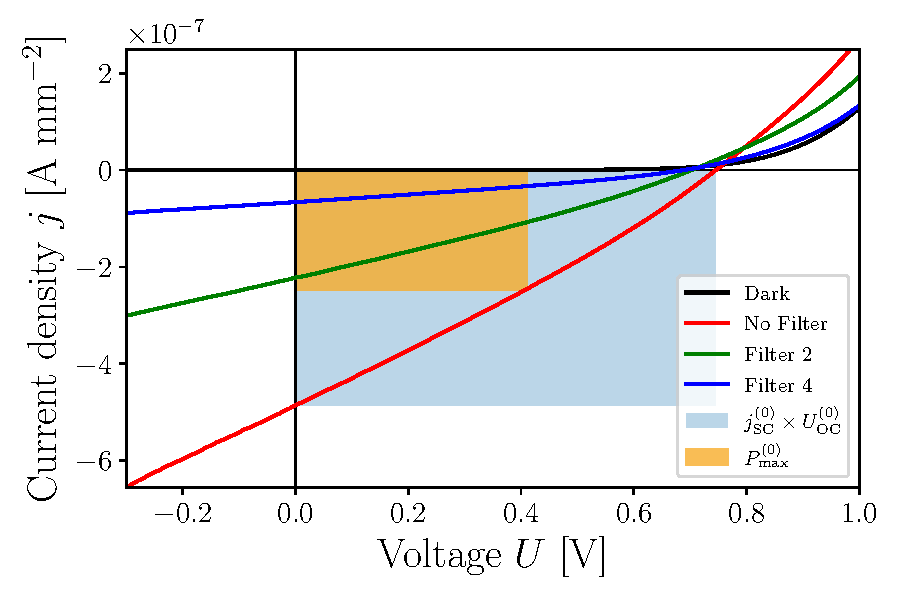
\includegraphics[width=\columnwidth]{../../../IV-Curve-Analysis/OSCPGraph.pdf}
\caption{Current density measurements for the set $\mathbb{S}_\star$}
\label{fig:OSCstarGraph}
\end{figure}

